\documentclass[10pt]{article}
\usepackage[margin=1in]{geometry}

\usepackage{biblatex}
\addbibresource{./references.bib}

\usepackage{hyperref}
\usepackage{xcolor}
\hypersetup{
    colorlinks,
    linkcolor={red!70!black},
    citecolor={blue!70!black},
    urlcolor={blue!90!black}
}

\usepackage{tikz}
\usetikzlibrary{shapes,arrows}

\begin{document}
This is an overview of the material point method.
While there are many variants due to the experimental nature of MPM, this document is focused on the current implementation.
For a more general review, please see the paper by \textcite{buzzi08}.

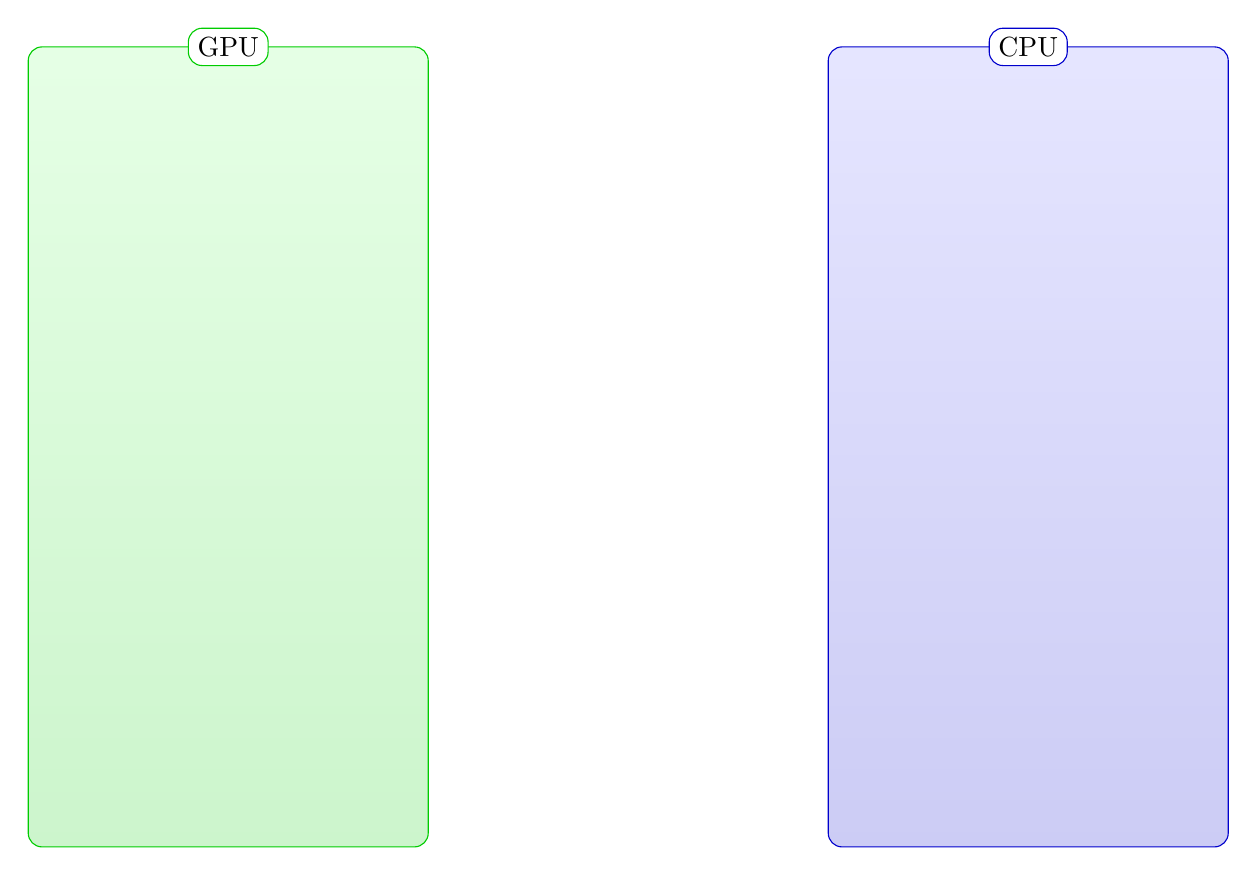
\begin{tikzpicture}
\tikzstyle{gpuborder}=[draw=green!80!black]
\tikzstyle{gpushade}=[shade, top color=green!10, bottom color=green!80!black!20]
\tikzstyle{ongpu}=[shade, top color=green!20, bottom color=green!70!black!20]
\tikzstyle{cpuborder}=[draw=blue!80!black]
\tikzstyle{cpushade}=[shade, top color=blue!10, bottom color=blue!80!black!20]
\node (A) at (0.5, 1) {Test};
\path[gpushade, gpuborder, rounded corners=5pt] (0, 0) -- (0, 4in) -- (2in, 4in) node[pos=0.5, fill=white, gpuborder] {GPU} -- (2in, 0) -- cycle;
% \path[ongpu, gpuborder] (1in, 3in) -- (2in, 3in) -- (2in, 2in) -- cycle;
\path[cpushade, cpuborder, rounded corners=5pt] (4in, 0) -- (4in, 4in) -- (6in, 4in) node[pos=0.5, fill=white, cpuborder] {CPU} -- (6in, 0) -- cycle;
\end{tikzpicture}

\printbibliography

\end{document}
